\documentclass[onecolumn, draftclsnofoot,10pt, compsoc]{IEEEtran}
\usepackage{graphicx}
\usepackage{url}
\usepackage{setspace}
\usepackage[margin=0.75in]{geometry}
\setlength{\parindent}{0pt}
\usepackage[hidelinks]{hyperref}
\usepackage{listings}
\usepackage{float}

\renewcommand\thesection{\Roman{section}}
\renewcommand\thesubsection{\Alph{subsection}}
\renewcommand\thesubsubsection{\arabic{subsubsection}}

\usepackage{etoolbox}
\patchcmd{\thebibliography}{\refname}{}{}{}


\usepackage{geometry}
\geometry{textheight=9.5in, textwidth=7in}

% 1. Fill in these details
\def \CapstoneTeamName{		Aerolyzer}
\def \CapstoneTeamNumber{		22}
\def \GroupMemberOne{			E. Reilly Collins}
\def \GroupMemberTwo{			Sophia Liu}
\def \GroupMemberThree{			Jesse Hanson}
\def \CapstoneProjectName{		Aerosol Analyzer Mobile Web Application}
\def \CapstoneSponsorCompany{	NASA JPL}
\def \CapstoneSponsorPerson{		Kim Whitehall, Lewis McGibbney}

% 2. Uncomment the appropriate line below so that the document type works
\def \DocType{		%Problem Statement
				%Requirements Document
				%Technology Review
				Design Document
				%Progress Report
				}
			
\newcommand{\NameSigPair}[1]{\par
\makebox[2.75in][r]{#1} \hfil 	\makebox[3.25in]{\makebox[2.25in]{\hrulefill} \hfill		\makebox[.75in]{\hrulefill}}
\par\vspace{-12pt} \textit{\tiny\noindent
\makebox[2.75in]{} \hfil		\makebox[3.25in]{\makebox[2.25in][r]{Signature} \hfill	\makebox[.75in][r]{Date}}}}
% 3. If the document is not to be signed, uncomment the RENEWcommand below
\renewcommand{\NameSigPair}[1]{#1}

%%%%%%%%%%%%%%%%%%%%%%%%%%%%%%%%%%%%%%%
\begin{document}

\begin{flushleft}
\section*{Signatures}

\subsection*{Kim Whitehall\\Client, NASA JPL} % Suppress subsection numbering with the *

\begin{tabular}{ l p{10pt} l }
Signature: && \hspace{0.5cm} \makebox[3in]{\hrulefill} \\ \\[3pt]
Date: && \hspace{0.5cm} \today
\end{tabular}

\subsection*{Lewis McGibbney\\Client, NASA JPL} % Suppress subsection numbering with the *

\begin{tabular}{ l p{10pt} l }
Signature: && \hspace{0.5cm} \makebox[3in]{\hrulefill} \\ \\[3pt]
Date: && \hspace{0.5cm} \today
\end{tabular}

\subsection*{E. Reilly Collins\\Student, Oregon State}

\begin{tabular}{ l p{10pt} l }
Signature: && \hspace{0.5cm} \makebox[3in]{\hrulefill} \\ \\[3pt]
Date: && \hspace{0.5cm} \today
\end{tabular}

\subsection*{Sophia Liu\\Student, Oregon State}

\begin{tabular}{ l p{10pt} l }
Signature: && \hspace{0.5cm} \makebox[3in]{\hrulefill} \\ \\[3pt]
Date: && \hspace{0.5cm} \today
\end{tabular}

\subsection*{Jesse Hanson\\Student, Oregon State}

\begin{tabular}{ l p{10pt} l }
Signature: && \hspace{0.5cm} \makebox[3in]{\hrulefill} \\ \\[3pt]
Date: && \hspace{0.5cm} \today
\end{tabular}
\clearpage


\begin{titlepage}
    \pagenumbering{gobble}
    \begin{singlespace}
    	%\includegraphics[height=4cm]{coe_v_spot1}
        \hfill 
        % 4. If you have a logo, use this includegraphics command to put it on the coversheet.
        %\includegraphics[height=4cm]{CompanyLogo}   
        \par\vspace{.2in}
        \centering
        \scshape{
            \huge CS Capstone \DocType \par
            {\large\today}\par
            \vspace{.5in}
            \textbf{\Huge\CapstoneProjectName}\par
            \vfill
            {\large Prepared for}\par
            \Huge \CapstoneSponsorCompany\par
            \vspace{5pt}
            {\Large\NameSigPair{\CapstoneSponsorPerson}\par}
            {\large Prepared by }\par
            Group\CapstoneTeamNumber\par
            % 5. comment out the line below this one if you do not wish to name your team
            \CapstoneTeamName\par 
            \vspace{5pt}
            {\Large
                \NameSigPair{\GroupMemberOne}\par
                \NameSigPair{\GroupMemberTwo}\par
                \NameSigPair{\GroupMemberThree}\par
            }
            \vspace{20pt}
        }
        \begin{abstract}
        % 6. Fill in your abstract    
        	Aerolyzer is a mobile web application capable of processing visible images and inferring atmospheric phenomena to provide the general public with near-real time monitoring of aerosol conditions. 
            This document outlines the software design descriptions for the Aerolyzer mobile web application and acts as a representation of a software design to be used for communicating design information to stakeholders. 
            A written description of the Aerolyzer software product is provided. 
        \end{abstract}     
    \end{singlespace}
\end{titlepage}
\newpage
\pagenumbering{arabic}
\tableofcontents
% 7. uncomment this (if applicable). Consider adding a page break.
\clearpage
\listoffigures
\listoftables
\clearpage

\begin{table}[h!]
\caption{Revision history}\label{table:1}
\centering
\begin{tabular}{| p{2cm} | p{2cm} | p{5cm} | p{3cm} |}
\hline
\textbf{Date} & \textbf{Version} & \textbf{Description} & \textbf{Author} \\
\hline
25 Nov 2016 & 1.0 & Initial version of document & E. Reilly Collins\\
\hline
26 Nov 2016 & 1.0 & Added summary & Sophia Liu\\
\hline
28 Nov 2016 & 1.0 & Added Pylint and ExifRead sections & E. Reilly Collins\\
\hline
30 Nov 2016 & 1.0 & Added MySQL section & E. Reilly Collins\\
\hline
29 Nov 2016 & 1.0 & Added TravisCI and Coveralls sections & Sophia Liu\\
\hline
30 Nov 2016 & 1.0 & Added Sphinx and MISR sections & Jesse Hanson\\
\hline
30 Nov 2016 & 1.0 & Added Wunderground and Django sections & Sophia Liu\\
\hline
1 Dec 2016 & 1.0 & Added DropzoneJS section & Jesse Hanson\\
\hline
12 Jan 2017 & 1.0 & Updated database section & E. Reilly Collins\\
\hline
\end{tabular}
\end{table}

\clearpage
% 8. now you write!
\section{Introduction} 
This document describes the conceptual design of the Aerolyzer mobile web application, according to guidelines presented in the IEEE Std. 1016-2009 Recommended Practice for Software Design Descriptions (SDD). The software is a web-based mobile application project that enables users to discover information about aerosol content based on uploaded images.

\subsection{Purpose }
The purpose of this document is to communicate design information to stakeholders for the Aerolyzer mobile web application. Software design descriptions are provided in order to give the software development team overall guidance to the project’s architecture. 

\medskip

Furthermore, this document aims to specify the features and requirements of the Aerolyzer software. The reader of this software design document will gain a technical understanding of Aerolyzer's design and implemented functionality. 


\subsection{Scope }
This software will be a mobile web application for use by the general public. 
This application will be designed to uniquely utilize color distribution within an uploaded mobile image to identify features necessary for analyzing aerosol content. 
The end product will be a full mobile web app that employs an open source algorithm translating how the human brain interprets images using RGB values. 
Citizens in the general public will be able to quantify color in images and use the resulting data to determine current aerosol content. 

\medskip %use this between paragraphs within a section or subsection, keep empty lines above and below

More specifically, users will be able to upload an image of an outdoor scene taken on a mobile phone. 
The application will then give output detailing the current aerosol content of the atmosphere based on the uploaded image. 
This software will provide average citizens with near-real time monitoring of atmospheric conditions.

\subsection{Context}
The task of this project is to provide the general public with near-real time monitoring of aerosol conditions via a mobile web application.The web interface is aimed to give users knowledge about current atmospheric conditions, combined with meteorological and geo-related data, based on images they upload to the app. Additionally, collected user results will form a data set that can be useful for research concerning atmospheric aerosol content. 

\medskip

The intended audience for this document are engineers or other stakeholders (including developers, software testers, and team managers) directly involved in the development and maintenance of the Aerolyzer mobile web application. This document is intended to provide these users with an understanding of the software’s design and underlying functionality.

\subsection{Summary}
The user will use this application to see the aerosol content in the air. First the user will take a picture of the skyline, and upload the unfiltered picture in the Aerolyzer application. The application will then analyze the data from the picture, and find out the time, date, and location it was taken. It will then send a request to Wunderground, and MISR, and using an algorithm, analyze the aerosol content. This data will then be re-packaged and presented to the user. 

\clearpage

\section{References}
\bibliographystyle{IEEEtran}
\bibliography{Aerolyzer_Design.bib}

\section{Glossary}
\textbf{Aerosol} Minute particles suspended in the atmosphere. When these particles are sufficiently large, we notice their presence as they scatter and absorb sunlight. Their scattering of sunlight can reduce visibility (haze) and redden sunrises and sunsets. \cite{1}

\medskip

\textbf{EXIF/exif} Exchangeable image file format specifying the specs of digital/smartphone cameras.

\medskip

\textbf{MISR} Multi-angle Imaging SpectroRadiometer satellite. \cite{2}

\clearpage

\section{Design}

\subsection{Identified stakeholders and design concerns}
Stakeholders for this project consists of the development team and users (the general public). The development team's concerns include creating maintainable software and producing accurate results, while the users are concerned with having their images secured and safe, receiving accurate output, an easy to use mobile web interface, and quick responsiveness. 

\medskip

These concerns have been discussed and will be addressed in the final product by: utilizing tools for the coding environment that increase code maintainability; creating test cases that check aerosol content results against actual data to improve the core algorithm, in addition to using data sources that provide accurate image metadata and real-time atmospheric data; using a trusted and researched database management system to store user images; and combining existing tools with user experience research to create a simple, user-friendly interface that increases responsiveness.

\subsection{Design viewpoint - Resources}
The purpose of the Resources viewpoint is to model the characteristics and utilization of resources in a design subject. Key concerns for our project that are addressed in the following design views are creating maintainable software (Pylint, Sphinx) and creating test cases (Travis CI and Coveralls). These concerns will be used to evaluate the effectiveness of our design regarding this specific viewpoint.

\subsubsection{Design view - Sphinx}
\textbf{Introduction} Throughout the development of our application, our team requires the ability to create professional and informative documentation of our API documents.
In order to satisfy this requirement, our team will be making use of Sphinx - a python documentation generator. This documentation tool provides a multitude of different functions including the ability for  semantic markups, automatic links for citations, a built in glossary structure, and much more. \cite{17} Moreover, this technology is compatible with Python, which is an essential requirement for our documentation process.
Through its various functions, this technology will allow us to produce clear and concise documentation on our code and how to use our application. Furthermore, its output formats include HTML, LaTex, and several others, which will be useful in creating easily accessible and compatible documents for users of our application.

\medskip

\textbf{Design element - Sphinx functionality} Sphinx provides a documentation structure that is quick and easy to use, allowing its users to connect multiple files within a hierarchy of documents. The master document serves as a welcome page and contains a table of contents which users may customize to fit their needs. \cite{17} This ability will allow our team to develop both code and usage documentation in a way that is both professional and instructive. Moreover, it will make our documentation more readable and easily accessible to our users.

\medskip

\textbf{Design element - Sphinx style component}
In general, our team will be utilizing the default functionality and style aspects of Sphinx. Since this API is highly customizable, we plan to customize our documents in a way that follows standard IEEE guidelines. However, we will also be making use of the various tools that accompany this API, including semantic markups, glossary terms, automatic links for citations, etc. \cite{17}

\medskip

\textbf{Design element - Sphinx framework}
For the development of our application, our team will be making use of Sphinx version 1.4.9, which is currently their newest version in production. \cite{17} The Aerolyzer Github repository will contain the necessary code and documentation templates shortly.

\smallskip

\footnotesize Authored by Jesse Hanson
\normalsize

\bigskip

\subsubsection{Design view - Pylint} \ \\
\textbf{Introduction} Since our team will be using Python to implement the Aerolyzer web application, we need a style guide that is Python-specific.
An existing technology that would accomplish this aim is Pylint. Pylint is a tool that searches for style errors in Python code in order to enforce a coding standard. \cite{20} One goal for the Aerolyzer project is high readability: we want our code to be easily read and understood by every member of the development team. 
Another goal for the use of Pylint in our design is to be able to catch syntax errors in order to avoid bugs. 
Python uses indentation to denote blocks, and significant logic errors can arise when whitespace is accidentally misused. 
We want to avoid such errors and reduce time spent on bugs that have a quick fix. 
A final goal for technology used in our coding environment is ensuring maintainability. The Aerolyzer software should live beyond our senior capstone class; this means other programmers will potentially need to read and add to our code. The handover and upholding process will be much smoother for our client (and result in better-quality software) if all code follows a specific format that can be learned by future team members.

\medskip

\textbf{Design element - Pylint subprogram functionality} Pylint defines a default coding style and can also look for specified coding errors, as well as provide refactoring suggestions. 
The software tries to avoid false positives while attempting to detect “dangerous” code blocks. 
After analyzing the Python code, Pylint offers an overall grade for the code based on the amount and severity of warnings or errors. 
This tool will unify the Aerolyzer team’s coding practices in order to be more efficient, as well as to create maintainable code. 

\medskip

\textbf{Design element - Pylint Style component} Specific guidelines included in our Pylint file include using 4 spaces instead of tabs for indentation, enforcing a max line length of 100 characters, and checking the import order using isort (a feature of Pylint implemented using isort). Other than these specifications, we are utilizing the default Pylint configuration (pylintrc).

\medskip

\textbf{Design element - Specific Pylint framework} Our project will use Pylint version 1.6.4. The Aerolyzer Github repository contains our lint file, {\href{https://github.com/Aerolyzer/Aerolyzer/blob/master/aerolyzer_lint_file}{aerolyzer\_lint\_file}}. Usage for our Aerolyzer lint file is \texttt{pylint --rcfile=aerolyzer\_lint\_file}.

\smallskip

\footnotesize Authored by E. Reilly Collins
\normalsize

\bigskip

\subsubsection{Design view - Travis CI and Coveralls}
\textbf{Introduction} Testing the code base while developing it is crucial to solve bugs as the code is being developed so the code does not end up with a million of bugs in the end.  Since Aerolyzer is hosted on Github, TravisCI and Coveralls are the best options for our project. TravisCI is an open-source continuous integration service used to build and test software projects hosted on Github \cite{15}.  Github makes it really simple to integrate TravisCI into our project. Coveralls is a  web service to help track the code coverage over time, and ensure that all of the new code is fully covered \cite{16}. It is extremely useful to check to see what tests cover what code, and what needs to be changed to help reach as close to 100 percent coverage as possible.

\medskip

One goal we have is easy integration. We want to make sure that the technology we use can be easily integrated into our code base. Both TravisCI and Coveralls is compatible with Github, and easily integratable. Another goal is keeping our entire program open source. TravisCI and Coveralls are both open-source programs. This ensures that our program will live beyond this project, and other programmers can work on the code because it is open source.

\medskip

\textbf{Design element - TravisCI and Coveralls subprogram functionality} TravisCI triggers automatic builds to every change to the Github code base including all branches and pull requests. TravisCI is built on the ideas of continuous integration, so basically everytime a new feature or change is added, TravisCI will run all tests to make sure that they all pass and the new code did not break some other part of the code\cite{15}. Coveralls is a tool that goes along with TravisCI and helps gather even more information about the test that are being run. Using Coveralls there are individual file coverage reports, line by line coverage reports, and repository coverage reports \cite{16}. It adds even more knowledge about the test coverage on top of the testing that TravisCI does.

\medskip

\textbf{Design element -  TravisCI Build Environment}The .travis.yml file customizes the build environment\cite{15}. The file specifies that we are using Python, the versions 2.6, 2.7, 3.2, 3.3, 3.4, 3.5, 3.6, and to run coveralls at the end.

\smallskip

\footnotesize Authored by Sophia Liu
\normalsize

\bigskip

\subsubsection{Design rationale} \ \\
\textbf{Sphinx} Overall, the justification for our decision to use Sphinx as opposed to several other documentation generators is quite simple. First and foremost, Sphinx was recommended to us by our client in light of the fact that Sphinx is compatible with our code, seeing as it is a Python documentation generator. However, several other reasons also influenced our decision to use Sphinx. The customizability of this tool was greatly appealing to us, as it will allow us to develop the documents according to our own specifications, as well as according to the requirements of our client and our senior design course. Moreover, the tools that accompany the Sphinx documentation generator will allow us to more easily create professional and informative documents that will aid in our users’ understanding of our application.

\medskip

\textbf{Pylint } Justification for this decision is based on the many benefits of using Pylint discovered through dialogue with our client, as well as researching the tool's documentation. These include its ability to catch bugs ranging from small to serious, more easily provide our team with a unified coding style, and offer refactoring features. Furthermore, Pylint is freely available, currently maintained with no evidence of becoming obsolete \cite{20}, and has plenty of easily understood documentation. \cite{6} 

\medskip

Our team has spent some time in our development cycle to narrow down a coding style for the Aerolyzer project and configure our own lint file. The time we would spend completing a code analysis with Pylint is definitely not equal to the time our team would otherwise spend manually finding syntax and logic errors. This time tradeoff will be especially relevant for any team members unfamiliar with coding in Python.

\medskip

\textbf{TravisCI and Coveralls} Justification for this decision is based off of the goals and the parameters of our project. Since we are using Github, TravisCI and Coveralls are the best option for testing. They are easily integrated into Github which makes them very easy to use to our project. They both have fairly new versions, and are being well-maintained. Another great thing about these two tools is that they are both completely open-source which works great for our project \cite{15}. This aligns with one of our main goals to keep our project open-source so other people can eventually contribute and use our program.

\bigskip

\subsection{Design viewpoint - Dependency}
\subsubsection{Design view - Solr} \ \\
\textbf{Introduction} The Aerolyzer system will require use of a database management system to perform data retrieval through a query language, securely store data, allow for concurrent access by multiple users, and keep data backed-up. The DBMS we have selected is Apache Solr. The maintained storage will consist of uploaded landscape images and their associated metadata, meteorological data, and geo-related data. Access to this database is necessary for a range of users, including members of the Aerolyzer development team (for improving the core algorithm) and any researchers who would like to make use of our collected data. The database will need to be backed-up regularly in the event of data loss or other situation that required data recovery.

\medskip

\textbf{Design element - Solr data store} The database design is illustrated in Figure \ref{fig:mysql}. It is divided into 3 tables: the images table, a table for image data acquired via EXIF metadata extraction, geo-related data acquired via MISR, weather data acquired from Weather Underground, the core algorithm’s output acquired after running the core algorithm successfully and receiving output. The primary key in this Images table links it to the second table, the Gallery table. This table holds the foreign keys to both Images and Accounts table. The Accounts table will hold the account ID, the username, password, first name, last name, and email.


\begin{figure}[H]
\centering
  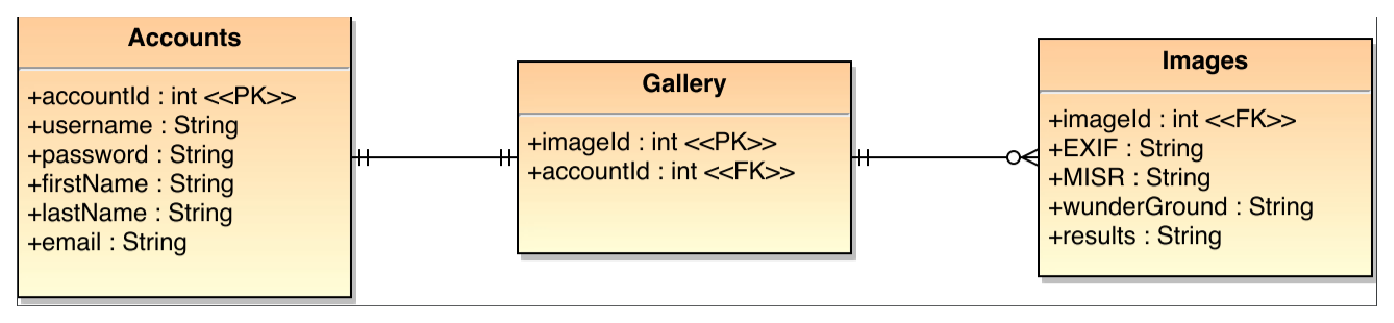
\includegraphics[width=\textwidth]{mysql.eps}
  \caption{Solr data store initial design}
  \label{fig:mysql}
\end{figure}


\textbf{Design element - Image\_Data entity} The image data entity will store image EXIF metadata. Currently, we are in the research phase of developing the core color-analyzing algorithm and therefore have not determined what specific EXIF metadata will be required. The specific database rows will be updated as the design of the algorithm is finalized. The \texttt{image\_id} is a primary key for the image across all entities. In addition, certain image metadata will be required as input for the core algorithm in order to produce results. Therefore, this entity is required.

\medskip

\textbf{Design element - Geo\_Data entity} Because we have not completed the design for the core algorithm, the data that will be pulled from the MISR source is still unknown. However, the specific rows containing geo-related data will be updated once the algorithm is designed. This entity is optional, as satellite data from MISR may not be available based on the image’s location. 

\medskip

\textbf{Design element - Weather\_Data entity} Required meteorological information for the core algorithm is more concrete at this point in the team’s research. Since we will be making use of the Weather API from Weather Underground, the team was able to determine what weather-related information is able to be extracted based on location information pulled from EXIF metadata. If other meteorological information is needed once the core algorithm has been designed, however, more rows will be added to this table. This entity is optional, as weather data from Weather Underground may not be available based on the image’s location. 

\medskip

As shown in Figure \ref{fig:mysql}, data for a specific image will be stored in multiple tables based on information extracted from different sources. The workflow will be similar to the following:
\begin{itemize}
\item  “SubjectLocation” EXIF tag will be pulled from an uploaded image’s metadata 
\item  Location is stored in the \texttt{Image\_Data} table
\item This location is used to determine the specific city and country the image was taken in via the Weather API
\item This city and country information is stored in the \texttt{Weather\_Data} table.
\end{itemize}

\medskip 

\textbf{Design element - Algorithm\_Data entity}
The core algorithm will use data from the other three entities as input and output aerosol content information. Currently, the core color-analyzing algorithm is being researched by the client stakeholder; as a result, the output of the algorithm (beyond the percentage of aerosol content) relating to atmospheric conditions is still unknown. Specific rows correlating to the output of the algorithm will be added to the database as needed. This entity is required, as any images that are stored in the \texttt{Image\_Date} table will have associated algorithm output that needs to be documented.

\smallskip

\footnotesize Authored by E. Reilly Collins

\normalsize

\bigskip


\subsubsection{Design rationale}
The Aerolyzer application will need a centralized storing location for images, associated metadata, and output from the color-analyzing core algorithm. Although we could make use of something simple, such as files in a shared directory, a database would be best suited for our needs: being able to maintain a repository of collected images and corresponding aerosol information will allow us to build up data for use in research, compare users’ results against real aerosol content, and query the data set for specific information that would be useful for our team and the research community. 

\medskip

The deciding factor for using Solr as a database management system was scalability. Comparisons using this criteria reveal that Solr is not only highly scalable, but is the best option for performing searches and even implements realtime search. \cite{5} Scalability will be very important for our app moving forward - we need to be able to store several pieces of data for each processed image and require searching for research purposes. Combining the scalability advantage with the fact that Solr is completely open source, stands behind the Apache brand, and supports data persistence makes it the ideal choice.

\subsection{Design viewpoint - Composition}
The purpose of the Composition viewpoint is to describe the way the design subject is (recursively) structured into constituent parts and establish the roles of those parts.  Key concerns for our project that are addressed in the following design views are obtaining accurate results both for the user and research purposes for the development team by using data sources that provide accurate image metadata and real-time atmospheric data. These concerns will be used to evaluate the effectiveness of our design regarding this specific viewpoint.

\subsubsection{Design view - Weather Underground}
\textbf{Introduction} In order to accurately analyze aerosol content in the pictures, it is important to have accurate real-time meteorological data. When users submit their pictures,the location and time is extracted . In order to get accurate aerosol information, the weather information is needed. The Weather Underground (Wunderground) API is the best tool to do this. The Weather Underground provides real-time temperature, air pressure, clouds, wind chill, dew point, humidity, and rainfall. They also provide radar maps. The radar maps can be either static or animated, depending on the call. The latitude and longitude is sent to the API, and it will return a radar map based on the call. \cite{3}

\medskip

\textbf{Design element - Weather Underground subprogram functionality} To use the API, the first required thing is to get an API key. Weather Underground API takes in a HTTP request, and returns either JSON or XML. We will then extract the data we need and use the information to help derive the Aerosol content in the air. \cite{3}

\medskip

\textbf{Design element - Specific Weather Underground Plan}To make our requests economical, we will be using the Stratus plan.  The Stratus plan only returns the information we need, so we do not need to sort through a large amount of data. This plan returns geolookup, autocomplete, current conditions, 3-day forecast, astronomy, and almanac for the day \cite{3}. To make the request even more efficient, we can specify the exact information we need, not just every thing that is returned in the Stratus plan. This will decrease the processing time from when the user uploads the photo, to when the user is returned the aerosol information based on their picture.

\smallskip

\footnotesize Authored by Sophia Liu
\normalsize

\bigskip

\subsubsection{Design view - MISR}

\textbf{Introduction} Seeing as the goal of our application is to accurately analyze the aerosol content of various images, we need the ability to obtain reliable and consistent geo-related data.
When searching for a technology that could satisfy this requirement, we focused on a few essential features. We need an API that is capable of obtaining truly accurate information on aerosol content, cloud formation, and light reflection. Moreover, this technology will need to be highly reliable and capable of continually supplying data, otherwise the accuracy of our results will suffer. 

\medskip

Therefore, to accomplish the task of obtaining geo-related data, we will be making use of NASA’s Multi-angle Imaging SpectroRadiometer (MISR). For all intents and purposes, MISR is an API which provides continual global coverage of the sunlit Earth in high spatial detail via nine widely spaced angles. \cite{2}

\medskip

Ultimately, we chose MISR as our technology for this task for a multitude of reasons. First and foremost, as a technology used by NASA, the accuracy of the data being provided will almost certainly be reliable. Along with this however, it is typically safe to say that the funding behind this API will be reliable enough to guarantee continual coverage.

\medskip

\textbf{Design element - MISR data extraction}
To gain access to the data provided by MISR, we must meet a minimum set of requirements according to NASA JPL. These requirements include EOSDIS Earthdata Login account, being CSS and Javascript enabled, and having HTML cookies enabled.
Once these requirements have been met, we will be able to make use of MISR visualization and analysis tools made available via MISR’s IDL data processing software package. This software package will include all of the necessary data processing software provided by the Atmospheric Sciences Data Center (ASDC) in production of data from MISR that is level 1 or higher. Moreover, it includes other tools such as data visualization and analysis used by MISR. \cite{24} 

\medskip

\textbf{Design element - MISR data customization}
Once we have access to the data provided by MISR, we will be able to uniquely order and customize the data we receive via MISR’s Order and Data Customization Tool. \cite{25} This will allow us to order customized level 2 data from MISR, as well as quickly download non-customized level 2 and level 3 MISR data. When used correctly, this tool will allow us to obtain more refined data according to specific dates, times, locations, etc.

\smallskip

\footnotesize Authored by Jesse Hanson
\normalsize

\bigskip



\subsubsection{Design view - ExifRead} \ \\
\textbf{Introduction} In order to ascertain aerosol content, the core color-analyzing algorithm needs an image's metadata as input. We are interested specifically in EXIF metadata that will provide the algorithm with needed information, such as the type of smartphone the image was taken on and the location of the photo. Having a wide range of information about uploaded images for the algorithm's input will in turn give output that is as accurate as possible. Our main goal regarding EXIF metadata extraction is to pull as much data from the image as possible. We will be making use of ExifRead, a technology that extracts all available EXIF data from an image, allowing us to use that data as input for the core algorithm. 


\medskip


\textbf{Design element - Required data for EXIF object} Currently, we are in the research phase of developing the core color-analyzing algorithm and therefore have not determined what specific EXIF metadata will be required. However, ExifRead is able to provide all standard EXIF metadata, so we can extract data corresponding to any tags we end up needing. An example of potential EXIF header data is listed in the UML diagram in Figure \ref{fig:exif}. \cite{21} This EXIF data will be pulled from uploaded images using the ExifRead package and stored in an object for use as input in the core algorithm. 

\begin{figure}[H]
\centering
  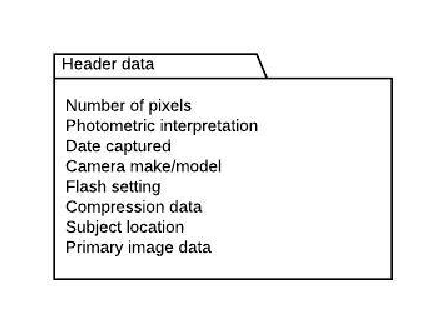
\includegraphics{exif.eps}
  \caption{Example EXIF metadata}
  \label{fig:exif}
\end{figure}

\textbf{Design element - EXIF extraction function} After installing the ExifRead Python package, the extraction of EXIF metadata will be accomplished via a function that stores the extracted EXIF data in an object using key-value pairs. This object can then be used as input for the core algorithm, and values can be accessed using keys as strings indicating the header data type using standard EXIF tags. This function will behave similar to the following code and result in an object similar to Figure \ref{fig:exif}: \cite{18} \ \\
\begin{lstlisting}
import exifread

# f: image to be processed
# Exif_Data: tuple to store EXIF data for current image
def get_exit_data(f, Exif_Data):

# Return EXIF tags
tags = exifread.process_file(f)

# Loop through tags and store required data in an object
for tag in tags.keys():
    if tag in ('SubjectLocation', 'PhotometricInterpretation', <etc>):
        cur_exif_data = Exif_Data(tag = tags[tag])
\end{lstlisting}
\smallskip
\footnotesize Authored by E. Reilly Collins
\normalsize

\bigskip

\subsubsection{Design view - DropzoneJS}
\textbf{Introduction} Since our application will ultimately allow users to analyze the aerosol content of various pictures, our web application requires the ability for users to upload images.
Our requirements for this technology are very simple. The API should be easy to use, while also allowing users to upload high quality images when may then analyze for aerosol content. We emphasis the necessity of high quality images because without this constraint, we would not be able to adequately analyze the content of the image being uploaded. Moreover, we need a technology that allows users to upload images both via a mobile device and from the web, and furthermore must be compatible with our code.

\medskip

To satisfy this requirement, we decided to go with the DropzoneJS. DropzoneJS is an open source library which does not rely on other libraries and is highly customizable. Moreover, it provides a simple drag and drop file upload and can be used programmatically. Finally, this API is ideal because it is compatible with most common browsers, including Chrome, Firefox, Internet Explorer (IE), and Safari. \cite{14}

\medskip

\textbf{Design element - DropzoneJS dropzone creation}
In order to begin uploading files, DropzoneJS first requires that a dropzone be created which can accept the file to be uploaded. There are a couple of ways in which we can go about this. Most commonly, dropzones are created as a form element via use of the class “dropzone”. From there, DropzoneJS will upload to that dropzone all images which are dropped into the action attribute of that form element. Alternatively, dropzones can be created programmatically by instantiating the Dropzone class, giving us some versatility in our implementation. \cite{14}

\medskip

\textbf{Design element - DropzoneJS drag and drop functionality}
One useful feature of DropzoneJS is its drag and drop functionality which allows users to drag and drop file directly into our web application for upload. This functionality can be set up programmatically; however, it is only supported recent versions of the most common browsers, including Firefox, IE, Chrome, Safari, etc. \cite{14} 

\medskip

\textbf{Design element - DropzoneJS server side implementation}
While DropzoneJS is simple, easy to use, and provides us with convenient dropzone creation and drag and drop functionality, it does not have server side implementation to determine how the uploaded files are handled. However, the file upload process is similar to that of a simple form file upload, therefore we can make use of several different server side implementations such as PHP to handle our files. \cite{14}

\smallskip

\footnotesize Authored by Jesse Hanson
\normalsize

\bigskip

\subsubsection{Design rationale} \ \\
\textbf{Weather Underground} Weather Underground is an accurate way to efficiently gather real-time meteorological data. The API is set up so data can be easily obtained. The only requirements are the location, which every picture will have since they are all taken on mobile devices. It also aligns with one of our big goals which is to keep this project open-source and free. Wunderground API is a free service so other developers can work on or use our code base.

\medskip

\textbf{MISR} Ultimately, MISR is the best technology available to us in terms of obtaining geo-related data for several reasons. As previously mentioned, since MISR is controlled by NASA JPL, the data provided by this technology will be both highly reliable and consistently provided. More specifically however, the data processing software packages provided by MISR and ASDC will be greatly beneficial to us as they will allow us to efficiently order and customize the data we receive. Along with this, we will have access to data visualization and analysis tools used by MISR, which will come in handy as we attempt to use this geo-related data to accurately analyze the aerosol content of various images.

\medskip

\textbf{ExifRead} The ExifRead package supports various versions of Python and returns GPS and manufacturer data in addition to standard EXIF metadata. \cite{18} GPS information will provide the core algorithm with additional meteorological data based on the image's location, and manufacturer data will be helpful for narrowing down the camera specs. It will be easy to use within our code, as it is a Python package, and we will not have to worry about storing our images in multiple locations:  EXIF metadata extraction can be done within the code rather than via an uploaded image. Lastly, as demonstrated in Figure \ref{fig:exif}, ExifRead will provide all of the metadata currently required of the Aerolyzer application.
\medskip

\textbf{DropzoneJS} While there are several available technologies for uploading files, we chose to go with DropzoneJS because its functionality best fit our application’s needs. The versatility of DropzoneJS in its creation of dropzones provides us with a couple of options in our development. Moreover, one of our criteria was to have a simple and easy to use file upload, which is made possible by DropzoneJS via its drag and drop functionality. Lastly, while we will have to develop our own server side implementation to determine how images are handled once uploaded, DropzoneJS is compatible with our code and will serve us well in making the first step of our application easily usable for our users.

\medskip

\subsection{Design viewpoint - Interface}
The purpose of the Interface viewpoint is to provide information for designers, programmers, and testers to know how to correctly use the services provided by a design subject. This section addresses design concerns of creating a simple, user-friendly interface that increases responsiveness. These concerns will be used to evaluate the effectiveness of our design regarding this specific viewpoint.

\subsubsection{Design view - Django}\ \\
\textbf{Introduction} Frameworks are an invaluable resource for developing web applications. The purpose of a framework is to allow the application to be well structured, and allows for other developers to easily maintain or upgrade the application. The goal should allow for the developers to not have to focus on low-level details. The framework should also be a fullstack framework. A fullstack framework is a framework that covers all layers of the stack, this essentially means that it will help the application be developed more efficiently without having to develop any layer from scratch. \cite{8} Django is a high-level Python Web framework that "encourages rapid development and clean, pragmatic design." \cite{8} Django also has a lot of built in security features, web forms, and templates.

\medskip

\textbf{Design element - Django subprogram functionality} Django has built in features to help with database transactions and manipulations. This will be useful when we are inserting pictures and data into the database. Django also has a really nice templating system. These systems auto generate HTML to make it simpler to create web pages. These pages can still be changed to fit the needs of the application. We will need at least 2 pages, one for uploading the picture, and one for displaying the data. A very important feature of Django is it’s security features. Since users are uploading personal photos, security is very important because users will not upload personal information into an application that is not secure. Django has cross-site scripting protection, Cross site request forgery protection, SQL injection protection
, Clickjacking protection, and Host header validation. \cite{8} Security is a concern for many people, and Django is great at having a lot of built-in security features.

\smallskip
\footnotesize Authored by Sophia Liu
\normalsize

\bigskip

\subsubsection{Design rationale}
\textbf{Django}  Django also has a lot of built in security features, database manipulations, and templates. Security is key to make sure that nobody’s personal information or pictures gets taken. People will not use an application that has security flaws. The templating system is also very useful. Writing every HTML page from scratch is a lot of unnecessary work, so having the pages auto-generated is time-saving. The database manipulation will make inserting, deleting, and editing our SQL database a lot easier. Frameworks are designed to make developing easier, and Django does just that.
\medskip

\subsection{Design viewpoint - Algorithm}
The purpose of the Algorithm design viewpoint is to provide a detailed design description of operations (such as methods and functions), the internal details and logic of each design entity. This section addresses design concerns of the speed and accuracy of the core color-analyzing algorithm. These concerns will be used to evaluate the effectiveness of our design regarding this specific viewpoint.

\medskip

\subsubsection{Design view - Core color-analyzing algorithm} \ \\
Currently, the core color-analyzing algorithm is in the research and development stage being performed by the client stakeholder. The design and testing for this core algorithm is not available to the editors of this SDD, and therefore the design concerns of its speed and accuracy cannot be described in this document. 

\clearpage

\section{Requirements Matrix}
\begin{table}[h!]
\caption{Functional requirements in SRS and SDD}\label{table:2}
\centering
\begin{tabular}{| p{2cm} | p{5cm} | p{2cm} | p{4cm} |}
\hline
\textbf{SRS ref} & \textbf{Functional requirement} & \textbf{SDS ref} & \textbf{Design viewpoint}\\
\hline
III-B-1 & Web Application Interface & IV-E & Interface \\
\hline
III-B-2 & Upload Photo & IV-E & Interface \\
\hline
III-B-3 & Display of Aerosol Content & IV-C & Dependency \\
\hline
III-B-4 & Extract EXIF Information From Data & IV-D & Composition \\
\hline
III-B-5 & Using Weatherunderground API & IV-D & Composition \\
\hline
III-B-6 & Get Data From Satellite Source & IV-D & Composition \\
\hline
III-B-7 & Running the Core Algorithm & IV-F & Algorithm \\
\hline
\end{tabular}
\end{table}
\end{flushleft}
\end{document}
